\chapter{Fundamentos teóricos de juegos y póker}

\section{Gestión de la información en los juegos: Juegos de Información perfecta y Juegos de información Imperfecta}
\label{sec:info}

En apartados anteriores ya se ha mencionado los conceptos de información perfecta e información imperfecta relacionados con la teoría de juegos.\cite{Gametheory}
 Este concepto se utiliza como una forma de clasificar los juegos extensivos.

Se define como juego extensivo a la descripción explícita de la estructura secuencial de la decisión de los problemas encontrados por los jugadores en una situación estratégica, permitiendo a cada uno de los jugadores considerar su estrategia y acciones a tomar no solamente al comienzo de la partida, sino que también permite considerar su plan de acción en cualquier momento en el que tenga que hacer una decisión. \cite{Gametheory}

Habiendo definido lo que es un juego extensivo, se puede hacer la clasificación según la información. 

Se considera que un juego tiene información perfecta cuando, a la hora de tomar una decisión dentro de una partida, el jugador tiene información de todos los eventos que han ocurrido previamente y conoce al completo el estado de juego actual. Un juego extensivo con información perfecta tiene los siguientes elementos:

\begin{itemize}
\item Un conjunto $N$, que corresponde al conjunto de jugadores.
\item Un conjunto $H$, que es el conjunto de historias, donde cada uno de los componentes de la historia es una acción tomada por un jugador. Este conjunto $H$ de secuencias (finitas o infinitas) debe cumplir las siguientes condiciones:
\begin{itemize}
\item La secuencia vacía $\emptyset$ pertenece a $H$. Esta historia es el punto inicial de la partida, llamado habitualmente \textit{historia inicial}.
\item Si $(a^k)_{k=1,...,K}\in H$, donde $K$ puede ser infinito, y siendo $L< K$, entonces $(a^k)_{k=1,...,L}\in H$.
\item Si una secuencia infinita $(a^k)^\infty_{k=1}$ cumple que $(a^k)_{k=1,...,L}\in H$ para cada valor positivo entero $L$, entonces  $(a^k)^\infty_{k=1}\in H$.
   \end{itemize}
\item La función jugador $P$, que asigna a cada historia que no sea terminal (es decir, a cada miembro de$ H\backslash  Z$) un miembro de $N$. siendo $P(h)$ el jugador que tiene que tomar una decisión tras la historia $h$.
\item Un conjunto $Z$, que incluye todas las historias terminales. Una historia $(a^k)_{k=1,...,K}\in H$ es terminal si es infinita o si no hay ningún $a^{K+1}$ que cumpla  $(a^k)_{k=1,...,K+1}\in H$.
\item La relación de preferencia del jugador $i$. Es decir, para cada jugador $i \in N$, una relación de preferencia $\succsim_i$ sobre $Z$.
\end{itemize} 

Si el conjunto $\langle N,H,P\rangle$    cumple las tres primeras condiciones de la definición, se denomina forma de juego extensivo con información perfecta. \cite{Gametheory}

Algunos ejemplos de juegos de información completa son el ajedrez, el Go, las damas o el tres en raya.

Es necesario distinguir información perfecta de información completa. La información completa implica el conocimiento común de las estrategias, tipos de jugador y jugadas futuras de cada uno de los jugadores. Un juego de información perfecta puede tener o no información completa.

Se considera que un juego tiene información imperfecta cuando, en el momento en que tenga que tomar una acción un jugador, ese jugador solo tiene información parcial sobre las acciones tomadas previamente y/o del estado actual del juego. Un juevo extensivo con información imperfecta tiene los siguientes elementos:
\begin{itemize}
\item Un conjunto $N$, que corresponde al conjunto de jugadores.
\item Un conjunto $H$, que es el conjunto de historias, donde cada uno de los componentes de la historia es una acción tomada por un jugador. Este conjunto $H$ de secuencias (finitas o infinitas) debe cumplir las siguientes condiciones:
\begin{itemize}
\item La secuencia vacía  $\emptyset$ pertenece a $H$. Esta historia es el punto inicial de la partida, llamado habitualmente \textit{historia inicial}.
\item Si $(a^k)_{k=1,...,K}\in H$, donde $K$ puede ser infinito, y siendo $L< K$, entonces $(a^k)_{k=1,...,L}\in H$.
\item Si una secuencia infinita $(a^k)^\infty_{k=1}$ cumple que $(a^k)_{k=1,...,L}\in H$ para cada valor positivo entero $L$, entonces  $(a^k)^\infty_{k=1}\in H$.
   \end{itemize}
\item La función jugador $P$, que asigna a cada historia que no sea terminal (es decir, a cada miembro de $ H\backslash  Z$) un miembro de N$ \cup \{c\}$. siendo $P(h)$ el jugador que tiene que tomar una decisión tras la historia $h$. Si$ P(h) = c$  entonces es la probabilida la que determina la acción tras la historia $h$.
\item Un conjunto $Z$, que incluye todas las historias terminales. Una historia $(a^k)_{k=1,...,K}\in H$ es terminal si es infinita o si no hay ningún $a^{K+1}$ que cumpla  $(a^k)_{k=1,...,K+1}\in H$.
\item El conjunto $A$ que incluye las acciones disponibles tras una historia no terminal h. $A(h)=\{a:(h,a) \in H \}$.
\item Una función $f_c$ que asocia a cada historia $h$ que que sea $ P(h) = c$ una medida de probabilidad $f_c(\cdot|h)$ en $A(h)$, donde cada una de las medidas de probabilidad es independiente de las demas medidas, siendo $f_c(a|h)$ la probabilidad de que a ocurra tras $h$.
\item Para cada jugador $ i \in N$ una partición de información $\mathcal{I}_i$ de $\{ h \in H:P(h) = i \} $ cumpliéndose que $A(h) = A(h')$ siendo $h$ y $h'$ miembros de la misma partición. Se denomina conjunto de información del jugador $i$ al conjunto $I_i \in \mathcal{I}_i$.  Para cada $I_i \in \mathcal{I}_i$ se llama $A(I_i)$ al conjunto $A(h)$ y $P(I_i)$ al conjunto $P(h)$
\item La relación de preferencia del jugador $i$. Es decir, para cada jugador $i \in N$, una relación de preferencia $\succsim_i$ en riesgo sobre $Z$, que puede ser representado como el valor esperado del resultado de una función definida en $Z$.
\end{itemize} 

Si el conjunto $\langle N,H,P, f_c,(\mathcal{I}_i)_{i \in N}\rangle$ cumple estas condiciones, se denomina forma de juego extensivo de información inperfecta. \cite{Gametheory}

El grado de información de la que dispone cada jugador viene dado por $\mathcal{I}_i$. Estas particiones de cada jugador son un principio de la partida, ya que cada jugador puede  distinguir entre diferentes historias de su partición sin necesidad de hacer cualquier inferencia sobre las acciones de los demás jugadores. A medida que la partida se desarrolle, un jugador puede ser capaz de hacer inferencias que precise la información que disponga, en función de las acciónes de los demás jugadores.\cite{Gametheory}

Los juegos de cartas donde cada jugador tenga cartas privadas (es decir, que sean cartas que los demás jugadores no conocen), tales como el póker, el mus, el bridge o el blackjack, son ejemplos de juegos de información imperfecta. En estos se combina la información pública (información conocida por todos los jugadores) como información privada (información conocida únicamente por el jugador), creando en ellos interés para ser considerados desde el punto de vista de la inteligencia artificial. En el siguiente apartado se hablará de estos juegos con un poco más de profundidad.

\section{Juegos de Cartas}
\label{sec:cartas}

Dado el interés que despertan los juegos de información imperfecta desde el punto de vista de la inteligencia artificial, se van a explicar las bases de algunos de estos juegos. En concreto, de los juegos de cartas mencionados en el apartado anterior. Estos juegos comparten que son juegos de cartas con apuestas, pero cada uno con sus propias reglas y peculiaridades.

\subsection{Póker}

El póker engloba a un conjunto de juegos de cartas con apuestas, que comparten similitudes en las reglas y, en concreto, comparten la forma de apostar. El póker se juega habitualmente usando la baraja francesa estándar\footnote{Barajas de 52 cartas agrupadas en cuatro palos de 13 cartas cada uno: Tréboles, Picas, Diamantes y Corazones. Las 13 cartas que componen cada palo son As, 2 al 10 y 3 figuras: Jota (J), Reina (Q) y Rey (K).}, aunque en algunas variaciones se utilizan también los comodines de las barajas (dando lugar a barajas de 54 cartas). 

Las diferentes variaciones de póker tienen un funcionamiento similiar. En cada ronda de una partida de póker, uno o varios jugadores tienen que hacer una apuesta inicial obligatoria llamada \textit{ciega} (en inglés, \textit{blind}), tras lo cual se reparten cartas a cada jugado. Se desarrolla la ronda de juego mediante rondas de apuestas, donde cada jugador puede tomar una de las acciones establecidas en el orden establecido en sentido horario desde el jugador inicial. El jugador a la derecha del jugador inicial de cada mano recibe el nombre de \textit{dealer}, que es el jugador que actúa el último en cada ronda de apuestas. El \textit{dealer} también se encarga de barajar y repartir las cartas en caso de que no haya una persona encargada de hacerlo.\cite{howto}
Las posibles acciones de apuesta son:
\begin{itemize}
\item \textit{Ver} la apuesta, que iguala la apuesta de ese jugador a la apuesta más alta de la mesa.
\begin{itemize}
\item En el caso de que no haya una apuesta por encima de las demás sin que se haya producido ninguna acción de \textit{ver}, \textit{ver} la apuesta significa no tomar acción hasta que haya una variación de apuestas. En esa situación, si todos los jugadores \textit{ven} la apuesta sin que se haya producido una variación de apuestas en esa ronda de apuestas, la ronda de apuestas se da por finalizada.
\end{itemize}
\item \textit{Subir} la apuesta (aumentando su apuesta hasta una cantidad a su elección siempre que supere a la apuesta más alta de la mesa).
\item \textit{Pasar} la apuesta. Si un jugador decide \textit{pasar} la apuesta, significa que se retira de esa ronda de juego y no puede apostar más hasta la siguiente ronda de juego. 
\end{itemize}

Una ronda de apuestas acaba cuando todos los jugadores han \textit{visto} la apuesta más alta o cuando sólo uno de los jugadores no ha \textit{pasado} durante la ronda de juego actual. En el primer caso, las apuestas se suman al bote de la ronda de juego, y se continua con dicha ronda de juego. En el segundo caso, el jugador que no ha \textit{pasado} sería el ganador de la ronda de juego.

Entre cada una de las rondas de apuestas, los jugadores desarrollan su jugada con las cartas disponibles, dependiendo de la modalidad.
Cuando acaban todas las rondas de apuestas de una ronda de juego, si quedan al menos 2 jugadores sin que hayan \textit{pasado}, se revelan las cartas y se comparan las jugadas construidas por estos jugadores y determinando el ganador de la ronda de juego.

El ganador de la ronda de juego se queda con todo el dinero del bote de esa ronda de juego.

El póker tiene muchas variaciones, pero las más habituales son las siguientes\cite{pokertypes, howto} :

\begin{itemize}
\item \textbf{Five-Cards Draw.} También conocido como \textbf{Cantrell Draw}. En cada ronda de juego de esta variante se reparten 5 cartas a cada jugador que, tras la primera ronda de apuestas, se podrán cambiar tantas cartas como se quieran de dicha mano (desde ninguna hasta las 5 cartas), llevando a una segunda y última ronda de apuestas. El Five Cards Draw es la variante considerada más sencilla de todas, que permite familiarizarse con el juego y aprender el funcionamiento del póker.
\item \textbf{Texas Hold'em.} La principal característica de esta modalidad de Póker es el reparto de cartas. Mientras que en el Five-Cards Draw se reparten cinco cartas ocultas a cada jugador, en el Texas Hold’em se reparten dos cartas ocultas a cada jugador y se revelan a todos los jugadores un total de cinco cartas a lo largo de las fases de juego, dejando la posibilidad a cada jugador de formar su mejor jugada de cinco cartas entre el total de siete cartas disponibles para cada jugador. Esta variante es conocida como una de las más populares de póker.
\item \textbf{Omaha Hold'em.} Conocido habitualmente como \textbf{Omaha}. Esta modalidad de póker es muy similar a Texas Hold'em, aunque con dos variaciones principales: cada jugador recibe 4 cartas ocultas en lugar de dos y la jugada de 5 cartas formada tiene que estar formada siempre por 3 de las 5 cartas comunes y por 2 de las 4 cartas de la mano. El resto del desarrollo de cada ronda de juego es prácticamente idéntico al de Texas Hold'em (como modificaciones en función de cada una de las submodallidades de Omaha).
\item \textbf{Seven-card Stud.} En esta modalidad, cada jugador recibe inicialmente 2 cartas ocultas y una visible, carta con la que se determina el jugador inicial. A medida que se desarrolla la ronda de juego, cada jugador va recibiendo cartas visibles y ocultas tras cada una de las rondas de apuestas, acabando con una mano de 7 cartas (3 ocultas y 4 visibles), con la que tiene que formar la mejor jugada posible de 5 cartas. El desarrollo se puede resumir en \textit{2 ocultas, 4 visibles y 1 oculta}, ya que es el orden en que se reciben las cartas que forman su mano.
\end{itemize}

\subsection{Mus}

El Mus es un juego de cartas con apuestas que se suele jugar entre 4 jugadores (agrupados en dos parejas), jugándose con una baraja española estándar\footnote{Barajas de 40 cartas agrupadas en cuatro palos de 10 cartas cada uno: Oros, Copas, Espadas y Bastos. Las 10 cartas que componen cada palo son As(1), 2 al 7 y 3 figuras: Sota (10), Caballo (11) y Rey (12).}. Al ser habitual el jugarse por parejas, cada uno de los miembros se posiciona en la mesa enfrente del otro, de manera que nunca puedan tener acción dos jugadores de la misma pareja.

\begin{figure}[h]
\centering
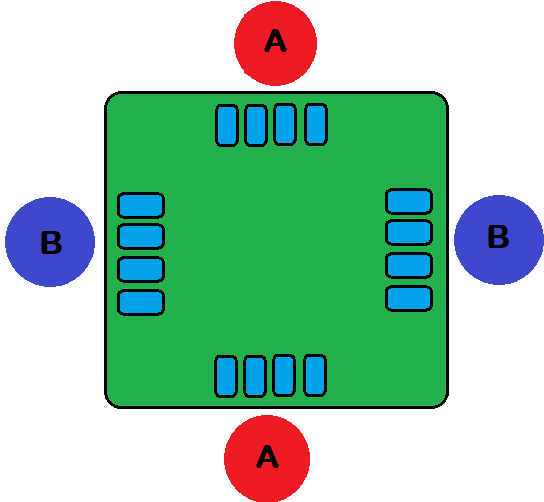
\includegraphics[width=0.75\textwidth]{figuras/Mus.png}   
\caption{Esquema de la distribución de los jugadores en una partida de Mus. \cite{propiaPaint}}
\label{fig:mus}
\end{figure}

La puntuación de cada carta (valor en torno al que gira todas las apuestas) varía según las variaciones de reglamento. Principalmente se consideran 2 versiones del reglamento. \cite{mus,mus2}
\begin{itemize}
\item \textbf{4 Reyes y 4 Ases.} Reglamento habitual en el Pais Vasco. Las cartas del As al 7 valen tantos puntos como número impreso en la carta (1-7) mientras que las figuras valen 10 puntos.
\item \textbf{8 Reyes y 8 Ases} Reglamento habitual en el resto de España. En este caso, los treses son equivalentes a los reyes (valiendo 10 puntos) y los doses son equivalentes a los ases (valiendo 1 punto). Al ser equivalentes, un tres y un Rey juntos forman una pareja, lo mismo que un As y un 2. El resto de valores es idéntico a la modalildad de 4 Reyes y 4 Ases.
\end{itemize}

Las figuras solo tienen el mismo valor para el lance de Juego/Punto, para el resto de lances tienen un orden de valor: Rey/Tres (en caso de 8 reyes)$>$Caballo$>$Sota.

Durante cada ronda de juego, llamadas \textit{manos}, se reparten 4 cartas a cada jugador, ocultas para los demás jugadores. Empezando por el jugador inicial, que también recibe el nombre de \textit{mano}, cada jugador decide si \textit{pide Mus}, es decir, diciendo si quiere cambiar alguna carta de su mano o si no quiere cambiar cartas de su mano (diciendo \textit{Mus} en caso de que quiera cambiar o  \textit{No hay mus} en caso de que no quiera). Si todos los jugadores piden Mus, empezando por el jugador que es mano descarta tantas cartas como quieran de su mano (siempre descartando, al menos, una carta) y recibiendo tantas cartas como haya descartado y se vuelve a preguntar a los jugadores si quieren Mus. En el momento en que un jugador no quiera Mus, comienzan las apuestas. \cite{mus}

Las apuestas, llamados \textit{envites}, durante cada una de las manos de Mus se dividen en 4 categorías, llamadas \textit{lances}. Los \textit{lances} de una partida de Mus son los siguientes (numerados por el orden en el que se realizan en cada ronda):
\begin{enumerate}
\item \textbf{Grande.} Cuanto mayor sea el valor de la combinación, mejor es la combinación para este lance. 
\item \textbf{Chica.} Cuanto menor sea el valor de la combinación, mejor es la combinación para este lance.
\item \textbf{Pares.} Cuantas más cartas del mismo valor y mayor sea ese valor, mejor es la combinación. Este lance solo se apostará si al menos un jugador de cada pareja tiene Pares.
\item \textbf{Juego /Punto.} En el lance de Juego, el objetivo es alcanzar 31 (siendo la mejor combinación para Juego) o superar 31 (cuanto mayor sea el valor en este caso, mejor). En caso de que ningún jugador supere los 31 puntos con las cartas que tienen, se apuesta por el lance de Punto. Para el lance de Punto, cuanto más se acerce el valor a 30, mejor es la combinación.
\end{enumerate}

Tras realizar los envites de todos los lances, se revelan las cartas y se determina qué pareja gana cada lance en el que se haya apostado, sumando los puntos apostados. Cuando una de las parejas alcance un número de puntos preacordado al comienzo de la partida (por lo general 30 ó 40 puntos), se acabará la partida, ganando esa partida la pareja con más puntuación.

A pesar de que cada jugador tenga sus 4 cartas y sean ocultas, si uno de los jugadores de la pareja gana un lance, la pareja como tal gana (ya que la puntuación de la partida se cuenta por pareja, no por jugador), lo cual fuerza a jugar con las cartas del compañero, pero manteniendo tus cartas ocultas para los oponentes. Para ello, es importante el uso de señas entre los miembros de una pareja para intentar comunicarse las jugadas que tienes.

\subsection{Bridge}

El Bridge\cite{bridge} es un juego de cartas de apuestas para 4 jugadpres que se juega con una baraja francesa estándar. Es juego se juega por parejas,  por lo que cada uno de los jugadores de la pareja se sienta enfrente de una manera equivalente a la vista en la figura \ref{fig:mus}. 

Lo más característico del Bridge es que la apuesta se hace es cuántas manos de una misma ronda puede ganar la pareja. Esta apuesta consiste en un número y un palo. El número indica cuantas manos por encima de 6 se pueden ganar, siendo el palo de triunfo el palo de la apuesta. En el caso de que se  haga una apuesta sin Triunfo, ningún palo será palo de triunfo. \cite{bridge}

El Bridge consiste de dos fases principales: el \textit{remate} y el \textit{carteo}.

Durante una partida de Bridge, uno de los jugadores baraja y reparte entre todos los jugadores todas las cartas del mazo, lo que da la comienzo al \textit{remate}. Esta ronda es la ronda de apuestas, en la que se tienen que apostar cuántas manos por encima de 6   El jugador que reparte se convierte en el primer subastador, que recibe el nombre de \textit{dador}. El dador puede hacer la apuesta o pasar al jugador de su izquierda.  \cite{bridge}

En el momento en que un jugador hace una apuesta, los demás jugadores pueden tomar una de las siguientes acciones:
\begin{itemize}
\item \textit{Ver} la apuesta.
\item \textit{Doblar} la apuesta, en el cual se sube al menos uno de los elementos de la apuesta (número o palo) hecha por la pareja oponente. En el caso de que el oponente haya doblado la apuesta, se considera que se \textit{redobla} la apuesta.
\item \textit{Pasar} la apuesta. 
\end{itemize} 

El número de la apuesta puede ir desde 1 (que significa que el apostante ganaría, al menos, 7 manos) hasta 7 (Que significa que el apostante ganaría las 13 manos).
La posibilidad de doblar el palo de la apuesta, hace que sea necesario establecer un orden de los palos.  El orden establecido es (de mayor a menor): Sin Triunfo, Picas, Corazones, Diamantes y Tréboles. 

A la hora de doblar es necesario quela nueva apuesta sea superior Una apuesta doblada puede mantener el mismo número pero aumentando el palo, al igual que si se aumenta el número de la apuesta, se puede poner cualquier palo como palo de triunfo. Es decir, que si la apuesta es  \textit{3 Diamantes}, se puede doblar la apuesta con  \textit{3 Picas}, al igual que con cualquier apuesta con un numero mayor a \textit{3}. Además, la única forma de doblar una apuesta con palo \textit{Sin Palo} es usando una apuesta de mayor número.\cite{bridge}

Cuando todos los jugadores han visto una apuesta, esta apuesta se la denomina como \textit{contrato}, y se asignan los papeles para la ronda del \textit{carteo}:
\begin{itemize}
\item El jugador que hizo el contrato se convierte en el  \textit{Declarante}.
\item La pareja del declarante se convierte en el \textit{Muerto}.
\item Los otros dos jugadores se convierten en los \textit{defensores}.
\end{itemize} 

En este momento comienza el \textit{carteo}. En esta fase es en la que se juegan las 13 manos de la ronda, en la cual el declarante tiene que ganar tantas manos como dice el contrato, mientras que los defensores intentarán evitarlo. 
La primera mano de esta fase la inicia el defensor sentado a la izquierda del declarante, que jugará una carta de su mano. Tras eso, el muerto muestra sus 13 cartas, colocándolas en el centro de la mesa ordenadas por palo y número. Estas cartas las jugará el declarante en cada una de las manos de esta ronda (por lo que el muerto no jugará el resto de la ronda). Una vez reveladas y ordenadas todas las cartas, el resto de jugadores tienen que jugar una carta del mismo palo que la carta inicial. En caso de no tener cartas del mismo palo, se puede jugar una carta de cualquier palo. \cite{bridge}

El ganador de la mano es el jugador que haya jugado la carta del palo inicial con el número más alto. La excepción a esto es el caso en que, al menos, un jugador haya jugado una carta del palo de triunfo (si lo hay). En esta situación, gana la mano el jugador que haya jugado la carta del palo de triunfo (en caso de que más de un jugador haya jugado una carta de ese palo, gana el jugador con la carta de triunfo de valor más alto).

El resto de las manos siguen este orden:

\begin{center}
 Defensor 1 $\rightarrow$ Declarante (usando las cartas del Muerto) $\rightarrow$ Defensor 2 $\rightarrow$ Declarante (con sus cartas).
\end{center}

Al final de la ronda, se cuentan las manos ganadas en una ronda. Si el declarante ha ganado las manos que apostó en el contrato, la pareja ganará tantos puntos según el número de la apuesta y el palo de triunfo de la misma.\cite{bridge}

\subsection{Blackjack}

El Blackjack \cite{blackjack} es un juego de apuestas que se usan barajas francesas estándar. Se puede jugar con una única baraja, pero lo habitual es mezclar barajas (siendo el más popular el de 6 barajas). 

En el Blackjack, el objetivo de los jugadores es conseguir sumar 21 puntos con las cartas de su mano, o quedarse lo más cerca posible sin pasarse. Así mismo, tienen que intentar superar a la jugada del crupier para ganar. Para esto, se suma el valor de las cartas de cada jugador. El valor de las cartas es el siguiente:
\begin{itemize}
\item 2-10: El valor de la carta
\item J,Q,K: 10 Puntos
\item A: 11 ó 1 Punto. Vale 11 puntos si la suma total no supera 21 o 1 en caso de que los supere.
\end{itemize} 

En el caso de que un jugador consiga una puntuación de 21 puntos con todas las cartas de su mano, se considera que ese jugador ha conseguido Blackjack.

En cada partida, se define un valor de apuesta fijo, que se mantiene salvo que se anuncie la subida de la apuesta. 
Al comienzo de la ronda, cada jugador coloca la apuesta fija delante suya y, despues de eso, el crupier reparte a cada jugador una carta bocarriba, y se reparte una carta a si mísmo bocarriba tambien. Tras eso, repite el proceso, con la salvedad de que la segunda carta del crupier suele ser oculta (dependiendo de las normas de la partida). Si la segunda carta del crupier es oculta, también lo es para el propio crupier.

Tras esto, es necesario comprobar si alguno de los jugadores tiene 21 natural, es decir,si su mano inicial incluye un As y una de las cartas de 10 puntos. En caso de que un jugador tenga un Blackjack natural, gana las fichas de los demas jugadores. En caso de que más de un jugador (crupier incluido) consiga Blackjack natural, se produce un empate, en la cual los jugadores con 21 recuperan su apuesta, y el resto de jugadores pierden lo apostado.

En la única situación en la que el crupier puede ver su carta antes de su turno es para comprobar si tiene un Blackjack Natural, es decir, solamente en caso de que su carta visible sea un As o una carta de 10 puntos.

Si ningún jugador tiene 21 natural, se comienza la ronda de apuestas. Empezando por el jugador más a la izquierda, cada jugador puede pedir una carta o plantarse. El jugador puede pedir cartas hasta que decida plantarse o hasta que se pase de 21. En el momento en que un jugador supere 21 puntos, pierde automáticamente, y el crupier toma la apuesta del perdedor. 

Cuando todos los jugadores hayan recibido cartas, es el turno del crupier de pedir cartas. Revela la carta bocabajo y toma la acción pertinente según la suma de sus cartas. Por lo general, está obligado a pedir carta mientras sume 16 o menos puntos, y a plantarse en cuanto sume 17 o más.

Una vez ha terminado el turno del crupier, se procede a hacer el recuento de los valores de los jugadores, en función del valor de la jugada del crupier y de los jugadores:
\begin{itemize}
\item Si el crupier se ha pasado de 21: Cada jugador recupera su apuesta y el crupier paga a cada jugador su apuesta.
\item Si el crupier tiene menos de 21 y ningún jugador ha conseguido Blackjack: Los jugadores que tengan menos puntuación que el crupier pierden su apuesta, y los jugadores que tengan más puntuación que el crupier recuperan su apuesta y el crupier les paga su apuesta.
\item Si el crupier y un jugador empatan: Ningún jugador pierde sus fichas ni recibe fichas.
\end{itemize} 

\begin{figure}[tb]
\centering
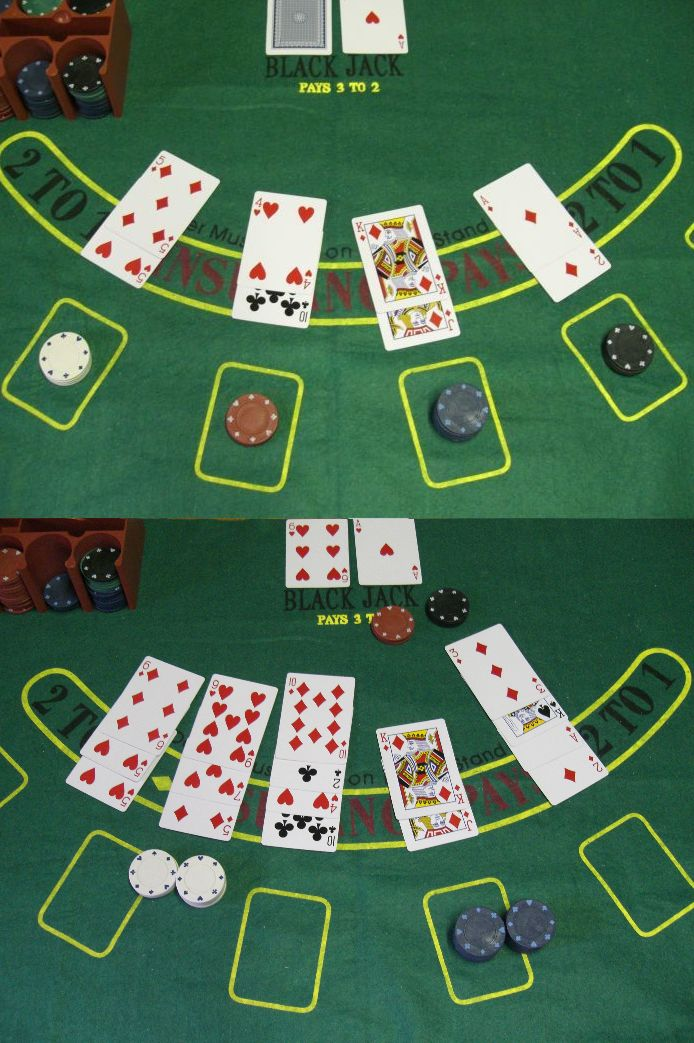
\includegraphics[width=0.5\textwidth]{figuras/blackjack.jpg}   
\caption{Ejemplo de una partida de Blackjack. En la imagen superior, se encuentra cómo es la partida antes de empezar el turno de los jugadores. En la imagen inferior, el resultado de la partida tras acabar la acción del Crupier.\cite{mesa}}
\label{fig:black}
\end{figure}


Además de pedir cartas o plantarse, los jugadores pueden tomar 3 opciones adicionales, pero estas opciones están limitadas a condiciones:
\begin{itemize}
\item \textbf{Separar:}Esta opción solo está disponible si las dos cartas iniciales del jugador son pareja. Separar permite al jugador dividir las cartas de su mano en dos apuestas al comienzo de su turno, siendo necesario apostar para la segunda mano. Por lo que queda de mano, cada una de las apuestas son tratadas como si fueran independientes.
\item \textbf{Doblar:} Esa acción permite al jugador pedir una única carta bocabajo, que se mantiene bocabajo hasta el final de la mano. Por lo general, solo se puede pedir esta acción si las cartas iniciales de ese jugador 9, 10 ó 11. 
\item \textbf{Asegurar:}Si la carta revelada del crupier es un As, los jugadores pueden apostar a Asegurar. Esto hace que el jugador apueste la mitad de su apuesta actual en el Seguro. En caso de que el crupier obtenga un Blackjack, la apuesta principal la sigue perdiendo, pero el jugador que haya apostado a Asegurar gana el doble de lo apostado en el Seguro.
\end{itemize} 

Por último, uno de los elementos mas importantes es el conteo de las cartas que han salido a lo largo de la partida, pues el mazo no se baraja al final de cada mano, sino que se baraja únicamente cuando se acaba el mazo. También baraja el mazo cuando acaba la ronda de juego.\cite{blackjack}

\section{Criterios para la elección de un juego de cartas}
\label{sec:choices}

Una vez expuestos algunos ejemplos que pueden ser sujeto de estudio, es necesario tomar la decisión de cuál centrarse en el proyecto. Para ello, se establecen los siguientes criterios a la hora de hacer la elección:
\begin{itemize}
\item Gestión de la información: Debido al interés que suscita desde el punto de vista de la inteligencia artificial, se busca un juego de información imperfecta. Además, que pueda manejar de manera eficiente y uniforme la información pública.
\item Complejidad del arbol de decisiones: Un arbol de decisiones complejo es consecuencia de un alto nivel de combinatoria de acciones, pues se generan muchos posibles estados en función de los estados de juego. Esta complejidad obliga a que la inteligencia artificial tenga que ser adaptable, siendo un punto de interés para su estudio. 
\item Individualización de la toma de decisiones: Una de los primeros factores que se quieren eliminar para poder desarrollar el estudio del juego es el factor externo de la colaboración. En otras palabras, se quiere eliminar la posibilidad de que la toma de decisiones dependa de la información de un jugador que no sea el oponente.
\item Dificultad de juego: Este critero sirve para medir como de complicado son las normas del juego. Un juego con reglas sencillas, fácil de aprender, pero complejo a la hora de dominarlo es el juego que mejor cumple este criterio.
\end{itemize} 

En base a estos criterios, se examinan los juegos susceptibles de análisis, es decir, los mencionados previamente en este proyecto:

\begin{itemize}
\item Go y ajedrez: a pesar de ser juegos con una altísima complejidad del arbol de decisiones(del orden de $10^{360}$ y del orden de $10^{123}$), al ser un juego de información perfecta, queda descartado.
\item Póker: El póker es un juego de información imperfecta, con una complejidad de arbol de decisiones bastante alta (variando según la modalidad), la toma de decisiones es individual y las reglas básicas comunes son sencillas. El póker si cumple los cuatro criterios.
\item Bridge: Este juego es un juego estrictamente por parejas, por lo que no cumple el criterio de individualización.
\item Mus: Si bien es cierto que este juego tiene modalidad de jugadores individuales, el juego más extendido es el juego por parejas, por lo que no cumpliría el criterio de individualización.Además de eso, el grado de complejidad del arbol de decisiones es bastante inferior al de los demás juegos mencionados aqui, por lo que tampoco cumpliría el de complejidad.
\item Blackjack: El Blackjack es un juego sencillo cuyas decisiones se toman de manera individual. El problema viene con la información y la complejidad. Si bien es un juego de información imperfecta, si se mantiene el mismo estado inicial que para otros juegos como póker (es decir, 2 jugadores con un solo mazo), disminuye drásticamente la complejidad del arbol de decisiones de este juego. Además, siguiendo el flujo de juego normal del Blackjack, el flujo de información no es uniforme, pues está ligado completamente a las acciones, incluso dando lugar a estados que son callejones sin salida. Por estos motivos no cumple estos dos criterios.
\end{itemize} 

De esta manera, el único juego que cumple los cuatro criterios es el póker, lo que lo convierte en el juego elegido.
A continuación se detalla cuál de las variaciones de póker es el juego elegido para ser objeto de estudio de este proyecto. Es necesario considerar algún criterio adicional  a los arriba mencionados, pues la individualización de la toma de decisiones no varía en las modalidades estudiadas, mientras que la dificultad de juego apenas varía entre las modalidades.
Los criterios  a considerar para discernir cuál es la variación de póker a elegir son los siguientes:
\begin{itemize}
\item Gestión de la información: Este criterio evalúa en este momento la cantidad de información pública y privada que presenta cada uno de los juegos. La cantidad de información pública es muy importante de cara a desarrollar una inteligencia artificial, pues permite definir con más precisión el estado de juego actual y ayuda a establecer una estrategia adecuada.
\item Complejidad del arbol de decisiones: Este criterio evalúa la cantidad de estados de juego y de toma de decisiones que posee el juego.
\item Adaptabilidad y versatilidad: Con este criterio se busca evaluar cómo de versátil es el flujo de juego para permitir a los jugadores una corrección de estrategia en función de la información conocida.
\item Limitaciones de juego: Con este criterio se quiere evaluar si existe alguna limitación a la hora de tomar decisiones, establecer estados o que se den callejones sin salida.
\end{itemize}

Con estos criterios, se procede a evaluar las cuatro variantes de póker mencionadas en este proyecto:
\begin{itemize}
\item Five-Cards Draw. El Five-Cards Draw no cumple  el criterio de la adaptabilidad (puesto que solo se dispone de una actualización de información, limitando las acciones de los jugadores. Además de eso, es el único de los cuatro que no tiene cartas como información pública, siendo la información conocida la apuesta del oponente y el número de cartas
\item Texas Hold'em. El Texas Hold'em cumple los 4 criterios. No tiene ninguna limitación adicional, tiene una gran cantidad de estados posibles ($5.56*10^{13}$)\footnotemark, es una de las dos versiones que más información pública tiene (5 cartas reveladas comunes), que se va incrementando durante la ronda, y un total de 4 rondas de apuestas donde poder corregir la estrategia en función de la información revelada.
\item Omaha Hold'em. Si bien el Omaha es el que tiene la mayor cantidad de estados posibles ($1.14 * 10^{18}$)\footnotemark[\value{footnote}] y tiene la misma información pública que el Texas Hold'em, la cantidad de información oculta es mayor (ya que es necesario considerar cada una de las cuatro cartas ocultas del otro jugador) y, además, se crea una limitación a la hora de formar la combinación de cartas (3 cartas de mesa y 2 de mano), lo cual hace que el criterio de Limitaciones de juego no se cumpla.
\item Seven-card Stud. El Seve-card Stud es el juego con mayor adaptabilidad y versatilidad de los 4, pues tiene 5 rondas de apuestas. Pero teniendo en cuenta que es más dificil modelar al oponente (ya que tiene menos información pública de cada oponente que el Omaha o el Texas Hold'em), y que tiene una limitación de juego, y es que la ordenación de jugadores no es secuencial entre rondas, pues el jugador inicial se decide por la carta más baja de las cartas reveladas), no cumple el criterio de Limitaciones de juego.
\end{itemize}

\footnotetext{El cálculo de estos estados posibles se ha realizado mediante una multiplicación de la combinatoria posible en cada uno de los juegos. Para Texas es $\binom{52}{2}*\binom{50}{2}*\binom{48}{3}*45*44 =5.56*10^{13}$, para Omaha es $\binom{52}{4}*\binom{48}{4}*\binom{44}{3}*43*42=1.14 * 10^{18}$ y para el Seven-card es $\binom{52}{7}*\binom{45}{7}=6.07*10^{15}$. El caso del Five-cards es particular, pues los estados varían en función de las cartas descartadas tras la primera ronda de apuestas, siendo el número de estados base $\binom{52}{5}*\binom{47}{5}=3.99*10^{12}$. }
El único que cumple simultáneamente los 4 criterios es el Texas Hold'em, lo que lo convierte en el juego elegido para este estudio.

\section{Fundamentos teóricos de póker Texas Hold'em}
\subsection{Desarrollo de las partidas: Apuestas y Fases de Juego}

En el Texas Hold'em\cite{howto} se reparte dos cartas a cada jugador como mano inicial, cartas ocultas para los demás jugadores, cartas que se van incrementando con las 5 cartas que se van revelando a lo largo de las rondas de apuestas posteriores a la inicial. Además de eso, al comienzo de cada una de las 3 rondas en las que se revelan cartas comunes, la carta superior del mazo es descartada. Esto se conoce como \textit{quemar} una carta\footnote{Este elemento se introdujo como un elemento de seguridad para evitar que en una partida real el crupier pueda favorecer a algún jugador, pero no tiene influencia alguna en la probabilidad. En el modelado se va a incluir únicamente por mantener el parecido con el juego real, pero es un elemento totalmente inócuo para el funcionamiento del simulador o del algoritmo.}. 

A pesar de que una partida de Texas hold’em podría tener hasta 22 jugadores iniciales (44 cartas repartidos a los jugadores, las 5 cartas reveladas y las 3 cartas quemadas), las partidas, tanto en casinos como en torneos, ocurren en mesas de 2 a 10 jugadores. Este límite está establecido con el fin de mantener el dinammismo de la partida, pues un aumento de jugadores ralentizaría el juego.

A lo largo de cada ronda, las cartas se van repartiendo y revelando a los jugadores, y tienen cuatro rondas de apuestas, en las que cada jugador debe tomar una de las acciones de apuestas posibles:
\begin{itemize}
\item \textbf{Ver} la apuesta. En inglés \textit{Call}, que iguala la apuesta de ese jugador a la apuesta más alta de la mesa.
\begin{itemize}
\item En el caso de que no haya una apuesta por encima de las demás sin que se haya producido ninguna acción de \textit{ver}, \textit{ver} la apuesta significa no tomar acción hasta que haya una variación de apuestas. En esa situación, si todos los jugadores \textit{ven} la apuesta sin que se haya producido una variación de apuestas en esa ronda de apuestas, la ronda de apuestas se da por finalizada. En este caso, la acción recibe el nombre de \textit{Check} en inglés.
\end{itemize}
\item \textbf{Subir} la apuesta. En inglés \textit{Raise}, esta acción permite aumentar la apuesta del jugador a una cantidad a su elección, siempre que la cantidad de la nueva apuesta sea superior a la apuesta más alta de la mesa.
\item \textbf{Pasar} la apuesta. En inglés \textit{Fold}, esta acción significa descartar la mano y retirarse de la ronda de juego. Esto implica que un jugador que \textit{pase} no puede apostar más hasta la siguiente ronda de juego. 
\end{itemize}

Cada jugador va realizando apuestas de manera secuencial hasta que todos los jugadores han visto la apuesta, o hasta que todos los jugadores pasan menos uno. En este caso, la ronda finaliza, y el jugador que no ha pasado recibe el total de lo apostado.\footnote{Los casinos suelen aplicar una comisión de un \% sobre el total de la apuesta. A esto se le conoce como \textit{rastrillo} o \textit{rake} en inglés. Debido a que es un elemento exclusivo de los casinos y no es un elemento del póker como tal, en el resto del proyecto no se va a tener en consideración ni se le hará mención.}  

Una vez explicado el funcionamiento de una ronda de apuestas, se procede a explicar las fases de cada ronda de juego.

Al comienzo de la ronda de juego, se entrega la posición de \textit{Dealer}\footnote{La traducción de Dealer es crupier y, en caso de que no haya una persona encargada del reparto, el crupier se hace cargo de repartir las cartas. Dado que el término crupier puede dar lugar a confusión, se mantendrá el término inglés a modo de nombre de la posición de este jugador} (representado por una ficha, conocida como \textit{button}) al jugador que le corresponde esa ronda. El \textit{button} se va rotando de jugador a jugador de manera secuencial: el jugador que ha sido jugador inicial en una ronda de juego, en la siguiente recibe el \textit{button} y el jugador a su izquierda se convierte en el jugador inicial de esa ronda.  El \textit{Dealer} es el jugador que está situado a la derecha del jugador inicial de la ronda, es decir, el \textit{Dealer} es el último jugador en tomar una decisión y apostar.

Tras eso, se hacen las apuestas ciegas, o \textit{Blind Bets}, que son apuestas obligatorias que dos jugadores concretos tienen que hacer en cada ronda antes de ver las cartas: la ciega pequeña o \textit{Small Bet}, que es apostada por el jugador a la izquierda del \textit{Dealer} y la ciega grande o \textit{Big Bet}\footnote{La ciega grande se utiliza como medida de beneficio en una partida de póker, siendo esta unidad el bb/partida, es decir, Ciega grande/partida }, que es apostada por el jugador a la izquierda del jugador que apuesta la ciega pequeña. Por lo general, la ciega grande es la apuesta mínima de la ronda y la ciega pequeña es la mitad de la ciega grande.

\begin{figure}[h]
\centering
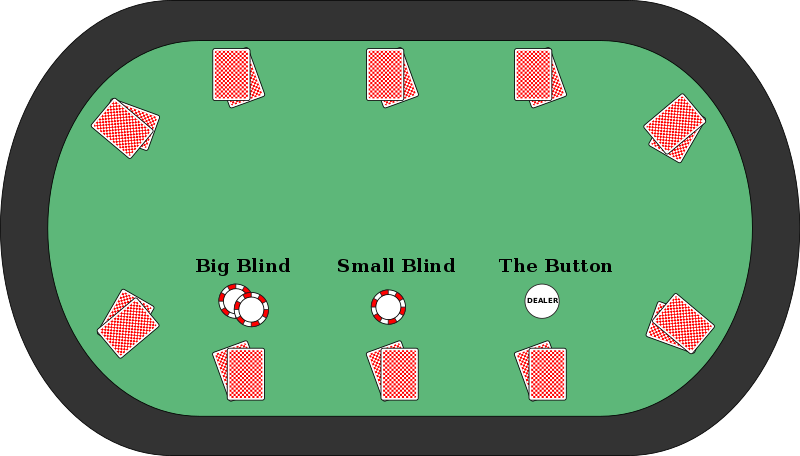
\includegraphics[width=0.90\textwidth]{figuras/Holdem_mesa.png}   
\caption{Diagrama de la distribución de las ciegas en cada partida.\cite{holdem_mesa}}
\label{fig:mesa_bids}
\end{figure}

Cuando una partida de Texas Hold'em avanza hasta el punto de que sólo queden dos jugadores en la partida, o en el caso de que se esté jugando en la modalidad \textit{heads-up} (partidas de dos jugadores), el jugador que sea el \textit{Dealer} tiene que realizar la ciega grande y el otro jugador (el jugador inicial) tiene que hacer la ciega pequeña.

Además de las apuestas ciegas, se pueden añadir apuestas obligatorias a todos los jugadores conocidos como \textit{Ante}, que es una apuesta obligatoria a todos los jugadores adicional a las apuestas ciegas para forzar a todos los jugadores a tener que arriesgar algo de dinero en cada ronda. En los torneos competitivos, tanto las apuestas ciegas como los \textit{Antes} van incrementándose a medida que el torneo avanza.\footnote{Al igual que pasa con el Rastrillo, los \textit{Antes} no se van a modelar, pues son un elemento añadido por los casinos y torneos.}

Una vez que el \textit{Dealer} ha sido designado y se han realizado las apuestas ciegas, cada jugador en la mesa recibe dos cartas boca abajo, llamadas \textit{Hole Cards} o \textit{Pocket Cards}, que serán las únicas cartas que recibirá cada jugador individualmente. 

Tras repartir las dos cartas a cada jugador, comienza la primera ronda de apuestas, conocida como \textbf{Preflop}. El primer jugador en apostar durante el \textbf{Preflop} es el jugador a la izquierda de la ciega grande. Tras acabar el \textbf{Preflop} y, si quedan al menos dos jugadores, se pasa a la siguiente fase. 

La siguiente ronda se llama \textbf{Flop}, en la que se quema una carta y se ponen tres cartas boca arriba en el centro de la mesa. Tras realizar el \textbf{Flop} se realiza una nueva ronda de apuestas, empezando por el jugador a la izquierda del \textit{Dealer}.


Una vez finalizada la ronda de apuestas del \textbf{Flop}, comienza la siguiente fase de la ronda, conocida como \textbf{Turn}.


Durante el \textbf{Turn} se quema la primera carta del mazo y después se revela una carta, que se coloca a la derecha de las tres cartas reveladas durante el \textbf{Flop}, siendo la cuarta carta revelada. Después de revelar la carta, comienza una nueva ronda de apuestas, empezando por el jugador a la izquierda del \textit{Dealer}.


Al acabar la ronda de apuestas del \textbf{Turn}, comienza la fase conocida como \textbf{River}, que tiene un funcionamiento similar a \textbf{Turn}: se quema la primera carta del mazo y se revela la siguiente carta del mazo, habiéndose revelado la quinta y última carta común a todos los jugadores. Tras revelar la carta, comienza la última ronda de apuestas, empezando por el jugador a la izquierda del \textit{Dealer}.


Al finalizar esta última ronda de apuestas, comienza la fase final de la ronda, conocida como \textbf{Showdown}. Durante el  \textbf{Showdown} cada jugador que siga en la ronda revela su mano y el jugador que tenga la mejor jugada gana, llevándose el total del dinero apostado (conocido también como \textit{pot}). Los tipos de jugadas y el orden deestas se explica en el apartado \ref{sec:class}.

Cabe destacar que el \textbf{Showdown} no siempre llega a suceder, ya que tiene que ocurrir que, al menos, dos jugadores terminen las  4 rondas de apuestas. Cuando no se llega al \textbf{Showdown}, el ganador es el único jugador que no haya pasado, independientemente de la mano que tenga.

\begin{figure}[h]
\centering
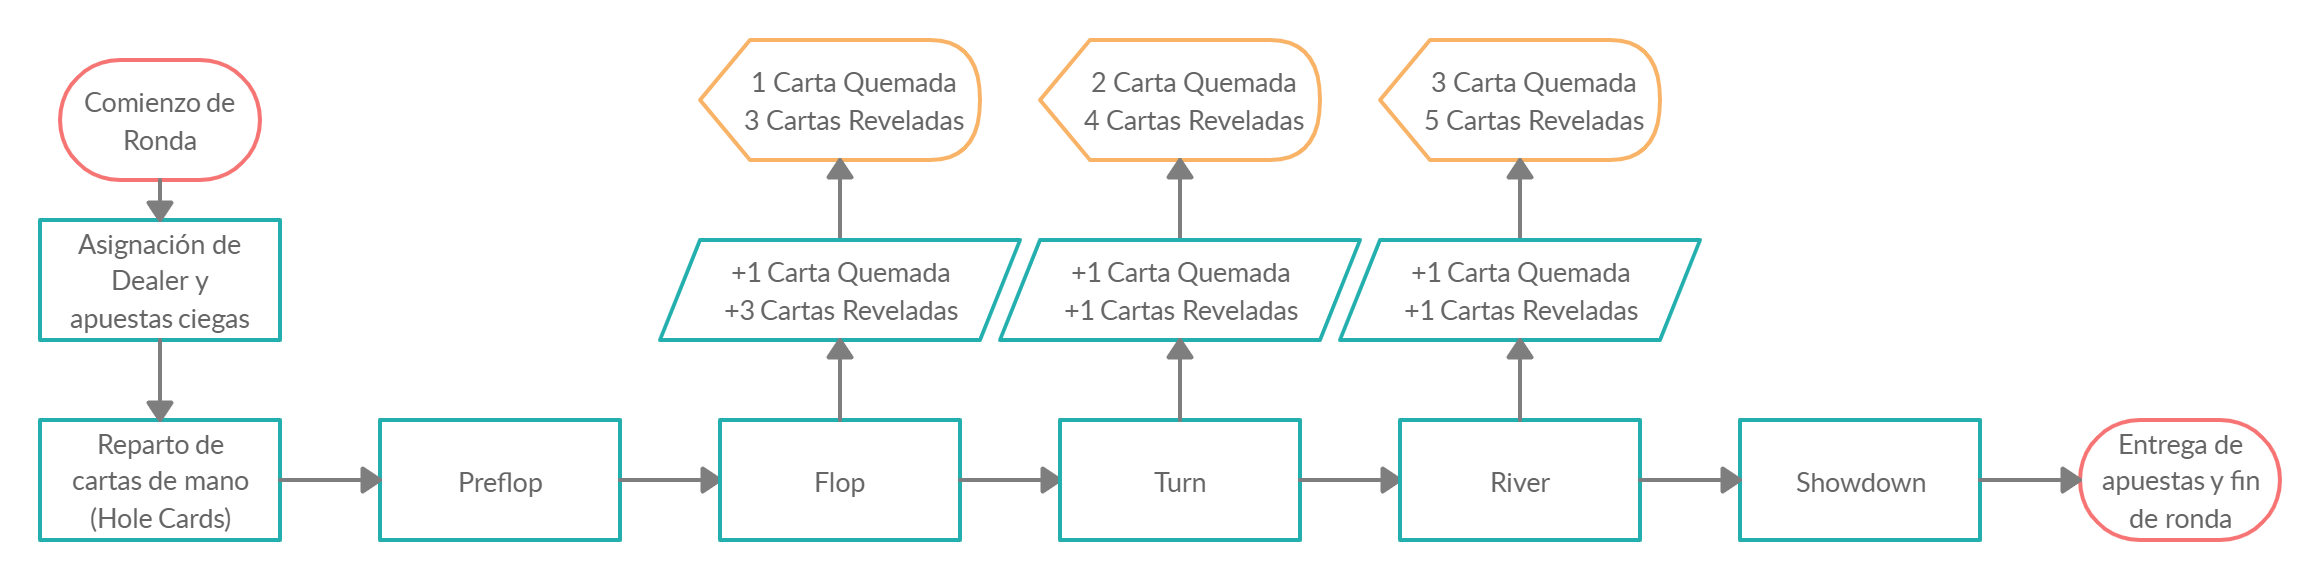
\includegraphics[width=0.9\textwidth]{figuras/Grafo3.png}   
\caption{Diagrama de la secuencia de una ronda de juego \cite{propiaCreately}}
\label{fig:bids}
\end{figure}

En resumen, el desarrollo de cada ronda de juego completa (suponiendo que, al menos, 2 jugadores apuestan en todas las rondas de apuestas) es el siguiente:
\begin{enumerate}
\item Entrega del \textit{Button}, apuestas ciegas y \textit{Antes} (en caso de que los haya)
\item Reparto de cartas iniciales (\textit{Hole Cards} o \textit{Pocket Cards})
\item Ronda de apuestas de \textbf{Preflop}
\item \textbf{Flop}: 1 carta quemada y 3 cartas reveladas.
\item Ronda de apuestas de \textbf{Flop}.
\item \textbf{Turn}: 1 carta quemada y 1 carta revelada.
\item Ronda de apuestas de \textbf{Turn}.
\item \textbf{River}: 1 carta quemada y 1 carta revelada.
\item Ronda de apuestas de \textbf{River}.
\item \textbf{Showdown}.
\end{enumerate}
 

\subsection{Clasificación de jugadas}
\label{sec:class}

Se conoce como jugada a la combinación de 5 cartas a partir de las cartas disponibles en una partida de Texas Hold'em tras el \textbf{Flop}. Los jugadores, durante la ronda de juego, formarán la mejor jugada con las 7 cartas que están a su disposición al final de la ronda, y compararán su jugada con la del resto de jugadores durante el \textbf{Showdown} . Para determinar la jugada, se han establecido las posibles jugadas, así como el orden de estas.  \cite{bridge}

Considerando que el número total de combinaciones es $\binom{52}{5}=$ 2.598.960, por lo que hay que tener en cuenta el número de posibles jugadas dentro del mísmo tipo. Estos datos se utilizarán en el apartado \ref{sec:prob_jug}, apartado en el que se calculará la probabilidad de cada una de las jugadas.

La siguiente tabla recoge las jugadas en orden descendente de valor, es decir, de la jugada más importante a la menos importante. 

\begin{longtable}[c]{|c|m{4em}|m{8em}|c|c|c|}
\hline
\rowcolor{lightgray} Orden & Nombre & Descripción & Ejemplo &  Freq.Absoluta & Frec.\\ \hline
1 & Escalera Real \textit{Royal Flush}&Cinco cartas del mismo palo del As al 10  &\textcolor{red}{A$\varheartsuit$K$\varheartsuit$Q$\varheartsuit$J$\varheartsuit$10$\varheartsuit$}& $\binom{4}{1}$ & 4 \\
\hline
2 & Escalera de Color \textit{Straight flush}&Cinco cartas consecutivas del mismo palo. En caso de empate, la carta más alta gana\footnotemark.  &9$\clubsuit$8$\clubsuit$7$\clubsuit$6$\clubsuit$5$\clubsuit$& $\binom{10}{1}\binom{4}{1}-\binom{4}{1}$ & 36 \\
\hline
3 & Póker \textit{ Four of a kind}&Cuatro cartas del mismo valor. En caso de que varios jugadores tengan póker, gana el póker de cartas más altas.  & \textcolor{red}{7$\varheartsuit$7$\vardiamondsuit$}7$\clubsuit$7$\spadesuit$2$\clubsuit$ & $\binom{13}{1}\binom{12}{1}\binom{4}{1}$ & 624 \\
\hline
4 & Full \textit{Full House}&Una combinación de un trío y una pareja. En caso de que varios jugadores tengan Full, gana el que tenga el trío más alto, y, en caso de que tengan el mismo trío, el que tenga la pareja más alta. &6$\clubsuit$6$\spadesuit$\textcolor{red}{6$\vardiamondsuit$10$\varheartsuit$}10$\clubsuit$ & $\binom{13}{1}\binom{4}{3}\binom{12}{1}\binom{4}{2}$ & 3.744 \\
\hline
5 & Color \textit{Flush}&Cinco cartas del mismo palo. En el caso de que varios jugadores tengan Color, gana el jugador con la carta más alta de ese palo.  & \textcolor{red}{K$\vardiamondsuit$8$\vardiamondsuit$7$\vardiamondsuit$6$\vardiamondsuit$4$\vardiamondsuit$}& $\binom{13}{5}\binom{4}{1} - \binom{10}{1}\binom{4}{1}$ & 5.108 \\
\hline
6 & Escalera \textit{Straight}&Cinco cartas consecutivas de palos diferentes. En caso de que varios jugadores tengan Escalera, gana el jugador con la carta más alta de la escalera.\footnotemark[\value{footnote}]& \textcolor{red}{Q$\vardiamondsuit$J$\varheartsuit$}10$\clubsuit$9$\spadesuit$8$\clubsuit$ & $\binom{10}{1}\binom{4}{1}^5- \binom{10}{1}\binom{4}{1}$ & 10.200 \\
\hline
7 & Trío \textit{Three of a kind}&Tres cartas del mismo valor. En caso de que varios jugadores tengan Trio, gana el Trio de mayor valor & \textcolor{red}{7$\varheartsuit$7$\vardiamondsuit$}7$\clubsuit$K$\spadesuit$2$\clubsuit$ & $\binom{13}{1}\binom{4}{3}\binom{12}{2}\binom{4}{1}^2$ & 54.912 \\
\hline
8 & Doble Pareja \textit{Two Pair}&Dos parejas de cartas. En caso de que varios jugadores tengan Dobles Parejas, gana el jugador con la pareja más alta, en caso de que tengan la misma pareja alta, gana el jugador con la segunda pareja más alta. & 8$\spadesuit$8$\clubsuit$6$\spadesuit$\textcolor{red}{6$\varheartsuit$2$\vardiamondsuit$} & $\binom{13}{2}\binom{4}{2}^2\binom{11}{1}\binom{4}{1}$ & 123.552 \\
\hline
9 & Pareja \textit{Pair}&Dos cartas del mismo valor. En caso de que varios jugadores tengan Pareja, gana el jugador con la pareja más alta.  & 7$\spadesuit$7$\clubsuit$K$\spadesuit$\textcolor{red}{4$\varheartsuit$}2$\spadesuit$  & $\binom{13}{1}\binom{4}{2}\binom{12}{3}\binom{4}{1}^3$ & 1.098.240 \\
\hline
10 & Carta Alta\textit{High Card}&La carta de mayor valor &\textcolor{red}{A$\varheartsuit$}10$\spadesuit$8$\clubsuit$7$\spadesuit$2$\clubsuit$ & $[\binom{13}{5}-10][\binom{4}{1}^5-4]$ & 1.302.540 \\
\hline
\caption{Clasificación de Jugadas en Texas Hold'em}
\label{tab:jugadas}
\end{longtable}

\footnotetext{Cabe destacar que, en las escaleras, el As puede tener un doble valor (As o 1), por lo que puede formarse tanto escalera de AKQJ10 como de 5432A. En este último caso, la carta más alta sería el 5. Únicamente ocurre esto con el As, haciendo que 5432A sea la única escalera posible que incluya cartas altas y bajas (Por ejemplo, 32AKQ no sería una escalera).}

En caso de que dos jugadores tengan exactamente la misma jugada, se aplica el valor de desempate, o \textit{kicker}, que es la carta de más valor fuera de la jugada sin importar su palo. Es decir, que si tu jugada es Q-Q-A-10-3, el \textit{kicker} sería A-10-3. En caso de tener la misma jugada, se empieza a comparar las cartas del \textit{kicker} y el que tenga la primera carta más alta que el \textit{kicker} del oponente, es el ganador.  En caso de que el \textit{kicker} sea idéntico, se produce un empate y se reparte el dinero acumulado de la apuesta entre los jugadores empatados.
Es importante tener en cuenta que hay jugadas en las que el \textit{kicker} no existe, ya que la jugada implica cinco cartas: Escalera Real, Escalera de Color, Full, Color y Escalera. 
También hay una posibilidad en la que el kicker no dependa de la mano del jugador, y es que las cartas más altas fuera de la jugada se encuentren en la mesa. Se expone un ejemplo de esto:
Quedan dos jugadores en la ronda durante el Showdown:
Jugador A: A$\spadesuit$\textcolor{red}{5$\vardiamondsuit$}
Jugador B: A$\clubsuit$10$\clubsuit$
Mesa: 2$\spadesuit$ \textcolor{red}{A$\varheartsuit$} K$\spadesuit$ \textcolor{red}{Q$\varheartsuit$ A$\vardiamondsuit$}
En este caso, la mejor jugada del jugador A es A$\spadesuit$ \textcolor{red}{A$\varheartsuit$A$\vardiamondsuit$}K$\spadesuit$ \textcolor{red}{Q$\varheartsuit$} mientras que la mejor jugada del jugador B es A$\clubsuit$ \textcolor{red}{A$\varheartsuit$A$\vardiamondsuit$} K$\spadesuit$ \textcolor{red}{Q$\varheartsuit$}. Es decir, que ambos jugadores tienen el mismo kicker a pesar de tener cartas de distinto valor en su mano, por tanto, se produciría un empate entre ambos jugadores.

\subsection{Faroles}
\label{sec:bluff}

Antes de tratar de los faroles, es necesario introducir los conceptos de \textit{draw} y \textit{Made Hand}. Un \textit{draw} es una mano de cuyo valor en caso de que la ronda terminara inmediatamente no sería la mejor de todas las posibles combinaciones entre las manos restantes, pero si salen determinadas cartas (llamadas \textit{outs}), mejora hasta ser la mejor. Es decir, es una mano que no vale nada a menos que salga una de sus outs, cartas que necesita para ganar. Mientras que \textit{Made Hand} es una jugada completa (Pareja, dobles parejas, Escalera…). Frente a un \textit{draw},\textit{Made Hand} suele apostar y subir. \cite{chen}

La causa de esta variación de valor de un \textit{draw} es el hecho de que el Texas Hold'em no es un juego estático, pues información se revela y eso provoca estos cambios de valores. 

Cuando la información es asimétrica, el jugador con\textit{Made Hand} está en desventaja ya que tiene que correr riesgos en algunas de las ocasiones en las que el \textit{draw} evidente aparece. En el caso de no correr esos riesgos, los demas jugadores pueden aprovecharse del \textit{draw} usando faroles de manera agresiva.\cite{chen}

Un farol, o \textit{bluff}, es una apuesta cuando la jugada que se tiene no vale nada. En otras palabras, un farol consiste en intentar intimidar a los demas mostrando una seguridad sin una jugada que la respalde.

Los faroles son una parte intrínseca de la psicología del póker, dado que un farol puede resultar en una gran pérdida de dinero cuando se resuelve. En torno a los faroles se pueden distinguir:\cite{chen}
\begin{itemize}
\item \textbf{Farol Puro:} es una apuesta con una mano que no tiene posibilidad alguna de ganar el bote mediante una estrategia óptima del oponente. Por lo general esto ocurre en las últimas fases de la ronda, donde la mano no puede mejorar.
\item \textbf{Semifarol:} es una apuesta con una mano que pueda o no ser mejor en el momento, pero puede mejorar tremendamente en las fases posteriores.
\item \textbf{Snowing:} Es un farol puro que se hace cuando no se tiene esperanza de ganar el bote en las primeras rondas de la partida.
\item \textbf{Apuestas de valor / Value bets:} Son apuestas que se espera que tengan una expectación positiva, incluso cuando son vistas. En casos extremos, incluso cuando un jugador tiene la mejor jugada posible en las primeras rondas, puede hacer una apuesta de valor pura en esas primeras fases, pero al igual que los faroles, es frecuente el caso de que, teniendo cartas pendientes de salir, la apuesta de valor pueda ser un semifarol (dependiendo de cómo de fuerte sea la mano del oponente). \cite{chen}
\end{itemize}